\section{The main problem}


\begin{frame}
  \frametitle[c]{The main problem}

  We want to present an inexact version of the scaled gradient projection method  for  \textcolor{UFGred}{constrained convex optimization problem} as follows

  \bigskip

  \begin{equation} \label{eq:OptP}
    \min \{ f(x) :~   x\in C\},
  \end{equation}

  \bigskip

  where $C$ is a closed and convex subset of $\mathbb{R}^n$ and $f:\mathbb{R}^n \to \mathbb{R}$ is a continuously differentiable function.
\end{frame}


\begin{frame}
  \frametitle{Scaled Gradient Projection Method\footfullcite{Bonettini2009}}

  \begin{enumerate}
    \item[Step 0.] Choose  $\sigma, \tau \in (0, 1)$, $0 < \alpha_{\min} \leq \alpha_{\max}$. Let $x^0\in C$ and set $k=0$;

    \item[Step 1.] Choose $\alpha_k\in [\alpha_{\min}, \alpha_{\max}]$ and a positive definite matrix $D_k$ and take  $w^{k}\in C$  as
      \begin{equation*}
        w^k := {\cal P}_{C}^{D_k} (x^{k}-\alpha_k D_k^{-1}\nabla f(x^{k}))
      \end{equation*}

      If $w^k= x^k$, then {\bf stop}; otherwise,
    \item [Step 2.] Choose $\tau_k$ and define the next iterate $x^{k+1}$ as
          \begin{equation} \label{eq:IterArm}
            x^{k+1} = x^{k} + \tau_k (w^k - x^{k}).
          \end{equation}
          and go back to the Step 1.
  \end{enumerate}
\end{frame}


\begin{frame}
  \frametitle{Scaled Gradient Projection Method}
  Let  $D$ be a $n\times n$ positive definite matrix and $\| \cdot \|_{D} : \mathbb{R}^{n}\rightarrow \mathbb{R}$ be  the norm  defined by
  \begin{equation*}
    \|d\|_{D}:=\sqrt{\left\langle D d,d\right\rangle},\quad \forall d\in \mathbb{R}^{n}.
  \end{equation*}
  For a fixed  constant $\mu \geq 1$,  {\it denote by  ${\cal D}_{\mu}$  the set of symmetric positive definite matrices $n\times n$ with all eigenvalues contained in the interval $[\frac{1}{\mu}, \mu]$}.
  \begin{itemize}
    \item ${\cal D}_{\mu}$   is compact;
    \item If $D\in {\cal D}_{\mu}$, it follows that $D^{-1}$ also belongs to $ {\cal D}_{\mu}$;
    \item $\forall D\in {\cal D}_{\mu}$,  we obtain
          \begin{equation*}
            \frac{1}{\mu}\|d\|^2\leq \|d\|^2_{D}\leq \mu \|d\|^2, \qquad \forall d\in \mathbb{R}^n.
          \end{equation*}
  \end{itemize}
\end{frame}


% \begin{frame}
%   \frametitle{Preliminaries}

%   \begin{definition}
%     Let $(y^k)_{k\in\mathbb{N}}$ be a sequence in $\mathbb{R}^n$ and   $(D_k)_{k\in\mathbb{N}}$ be  a sequence in ${\cal D}_{\mu}$.  The sequence $(y^k)_{k\in\mathbb{N}}$ is said to be \textcolor{UFGred}{quasi-Fej\'er convergent} to a set $W\subset \mathbb{R}^n$ with respect to  $(D_k)_{k\in\mathbb{N}}$ if, for  all $w\in W$, there exists a sequence $(\epsilon_k)_{k\in\mathbb{N}}\subset\mathbb{R}$ such that $\epsilon_k\geq 0$, $\displaystyle\sum_{k\in \mathbb{N}}\epsilon_k<\infty$, and
%     \[
%       \|y^{k+1}-w\|_{D_{k+1}}^2\leq \|y^k-w\|_{D_k}^2+\epsilon_k,
%     \]
%     for all $k\in \mathbb{N}$.
%   \end{definition}
% \end{frame}


% \begin{frame}
%   \frametitle{Preliminaries}

%   \begin{theorem}
%     Let $(y^k)_{k\in\mathbb{N}}$ be a sequence in $\mathbb{R}^n$ and   $(D_k)_{k\in\mathbb{N}}$ be  a sequence in ${\cal D}_{\mu}$.   If $(y^k)_{k\in\mathbb{N}}$ is quasi-Fej\'er convergent to a nomempty set $W\subset  \mathbb{R}^n$ with respect to $(D_k)_{k\in\mathbb{N}}$, then $(y^k)_{k\in\mathbb{N}}$ is \textcolor{UFGred}{bounded}. Furthermore, if a \textcolor{UFGred}{cluster point ${\bar y}$} of $(y^k)_{k\in\mathbb{N}}$ belongs to $W$, then $\displaystyle\lim_{k\rightarrow\infty}y^k={\bar y}$.
%   \end{theorem}
% \end{frame}

\section{Inexact Projections}

\begin{frame}
  \frametitle{Exact Projection}

  \begin{definition}[2.1]
    The \textcolor{UFGred}{exact  projection} of the point $v\in \mathbb{R}^{n}$ onto $C$ with respect to the norm $\| \cdot \| _{D}$, denoted by  ${\cal P}_{C}^{D}(v)$, is  defined~by
    \begin{equation*}
      {\cal P}_{C}^{D}(v):=\arg \min _{z\in C}\|z-v\|^2_{D}.
    \end{equation*}
  \end{definition}

  \begin{lemma}[2.2]
    Let $v, w \in {\mathbb R}^n$.  Then,  $w={\cal P}_{C}^{D}(v)$ if and only if  $w\in C$ and
    \[
      \left\langle D(v-w), y-w\right\rangle \leq  0,
    \]
    for all $y \in C.$
  \end{lemma}
\end{frame}

\begin{frame}[t]\frametitle{Exact Projection}\bigskip
  \begin{figure}[!ht]
    \centering
    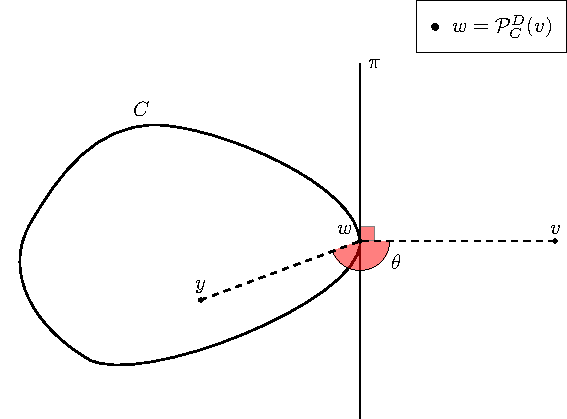
\includegraphics{../figures/exactProj.pdf}
    \caption{Exact projection of the point $v$ onto $C$.}
    \label{fig:exactProj}
  \end{figure}
\end{frame}


\begin{frame}
  \frametitle{Inexact Projections\footfullcite{BirginMartinezRaydan2003}}

  \begin{definition}[2.5]
    The \textcolor{UFGred}{feasible inexact projection mapping}, with respect to the norm $\| \cdot \|_{D}$,   onto $C$  relative to a point  $u \in C$ and forcing parameter $\zeta\in (0, 1]$, denoted by ${\cal P}_{C,\zeta}^{D}(u,  \cdot): {\mathbb R}^n \rightrightarrows C$,  is the set-valued mapping defined as follows
    \begin{equation*}
      {\cal P}_{C,\zeta}^{D}(u, v) := \left\{w\in C:~ \|w-v\|_{D}^2\leq \zeta \| {\cal P}_{C}^{D}(v)-v\|_{D}^2+(1-\zeta)\|u-v\|_{D}^2 \right\}.
    \end{equation*}
    Each point $w\in {\cal P}_{C,\zeta}^{D}(u, v) $ is called a  \textcolor{UFGred}{feasible inexact projection},  with respect to the norm $\| \cdot \|_{D}$,  of $v$ onto $C$ relative to $u$ and forcing parameter $\zeta\in (0, 1]$.
  \end{definition}
\end{frame}

\begin{frame}[t]\frametitle{Inexact Projections}\bigskip
  \begin{figure}[H]
    \centering
    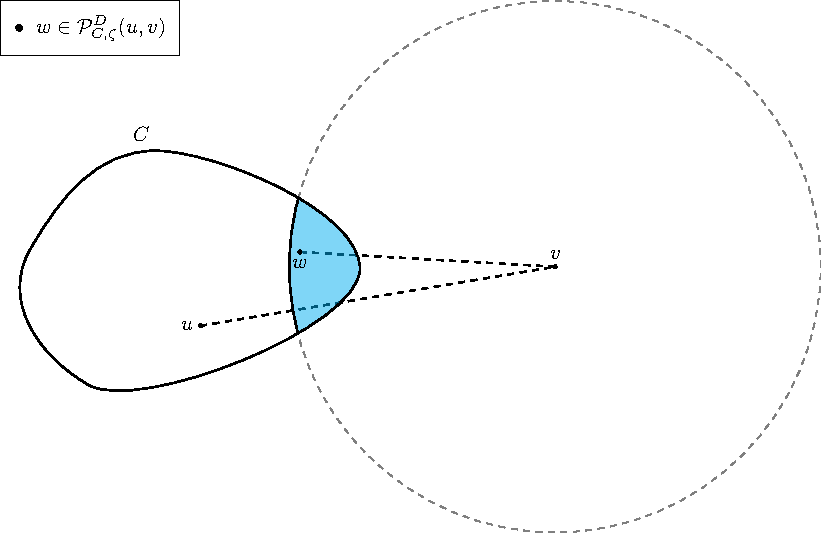
\includegraphics[height=0.725\textheight]{../figures/martinezProj.pdf}
    \caption{Feasible inexact projection of the point $v$ onto $C$.}
    \label{fig:martinezProj}
  \end{figure}
\end{frame}


\begin{frame}[t]\frametitle{Inexact Projections\footfullcite{OrizonFabianaGilson2018}}
  \begin{definition}[2.10]
    The \textcolor{UFGred}{feasible inexact projection mapping}, with respect to the norm $\| \cdot \|_{D}$,  onto $C$ relative to $u \in C$ and forcing parameter $\gamma\geq 0$, denoted by ${\cal R}_{C,\gamma}^{D}(u, \cdot): {\mathbb R}^n \rightrightarrows C$,  is the set-valued mapping defined as follows
    \begin{equation*}
      {\cal R}_{C,\gamma}^{D}(u, v):= \left\{w\in C:~\left\langle D(v-w), y-w \right\rangle \leq \gamma \|w-u\|_{D}^2, \quad \forall~ y \in C \right\}.
    \end{equation*}
    Each point $w\in {\cal R}_{C,\gamma}^{D}(u, v)$ is called a feasible inexact projection,  with respect to the norm $\| \cdot \|_{D}$,  of $v$ onto $C$ relative to $u$ and forcing parameter $\gamma\geq 0$.
  \end{definition}
\end{frame}

\begin{frame}[t]\frametitle{Inexact Projections}\bigskip   
  \begin{figure}[H]
  %\begin{adjustwidth}{2.2cm}{2.2cm}
  \begin{subfigmatrix}{2}
    \subfigure[Geometric interpretation.]{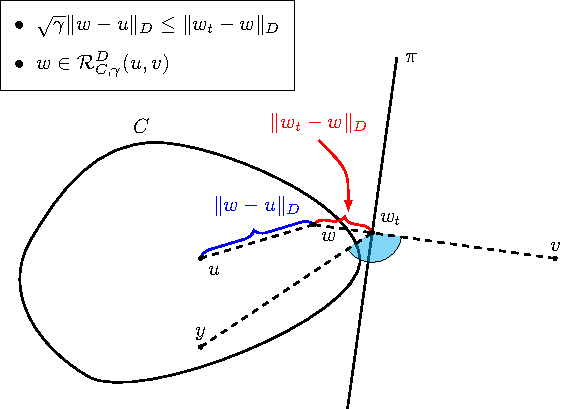
\includegraphics{../figures/condProj1.pdf}}
    \subfigure[Example of ${\cal R}_{C,\gamma}^{D}(u, v)$.]{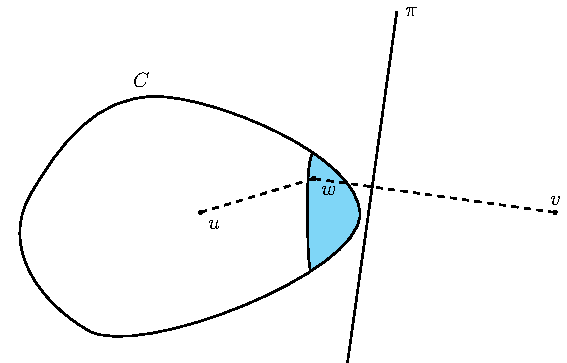
\includegraphics{../figures/condProj2.pdf}}
  \end{subfigmatrix}
  \caption{Geometric interpretation of projection ${\cal R}_{C,\gamma}^{D}(u, v)$.}
  \label{fig:condProj1}
  %\end{adjustwidth}
\end{figure}
\end{frame}

\begin{frame}[t]\frametitle{Inexact Projections}\bigskip   
\begin{figure}[H]
  %\begin{adjustwidth}{2.2cm}{2.2cm}
  \begin{subfigmatrix}{3}
    \subfigure[]{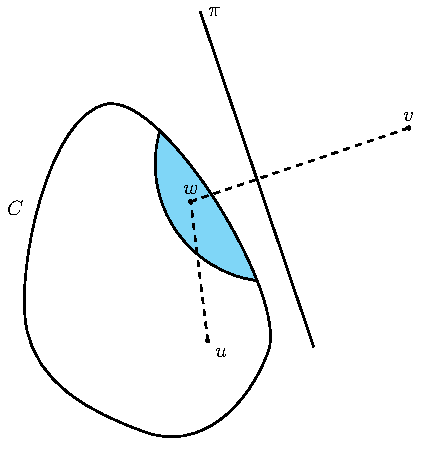
\includegraphics{../figures/condProj3.pdf}}
    \subfigure[]{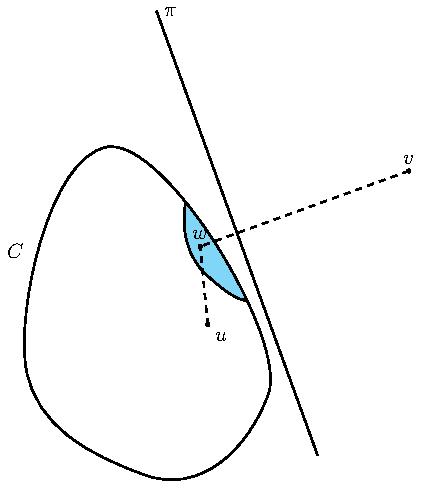
\includegraphics{../figures/condProj4.pdf}}
    \subfigure[]{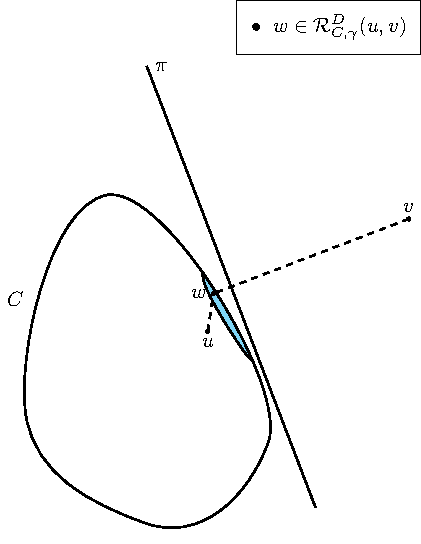
\includegraphics{../figures/condProj5.pdf}}
  \end{subfigmatrix}
  \caption{Examples of regions given by inexact projection ${\cal R}_{C,\gamma}^{D}(u, v)$.}
  \label{fig:baseline}
  %\end{adjustwidth}
\end{figure}
\end{frame}

\begin{frame}[t]\frametitle{Inexact Projections}\bigskip   
\begin{figure}[H]
  \begin{subfigmatrix}{3}
    \subfigure[]{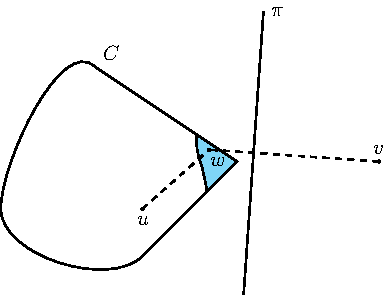
\includegraphics[width=0.3\textwidth]{../figures/condProj6.pdf}}
    \subfigure[]{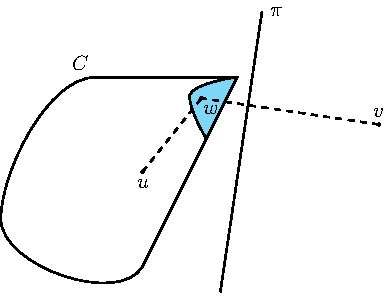
\includegraphics[width=0.3\textwidth]{../figures/condProj7.pdf}}
    \subfigure[]{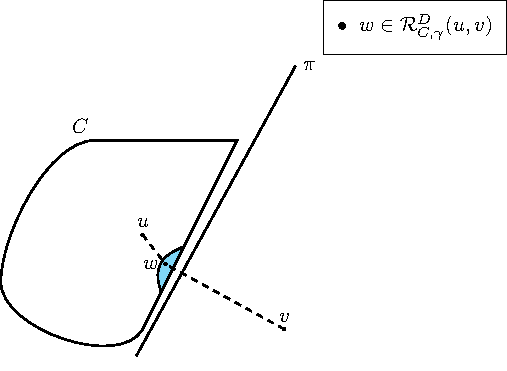
\includegraphics[width=0.37\textwidth]{../figures/condProj8.pdf}}
  \end{subfigmatrix}
  \caption{Examples of regions given by inexact projection ${\cal R}_{C,\gamma}^{D}(u, v)$.}
  \label{fig:baseline}
\end{figure}
\end{frame}


\begin{frame}[t]\frametitle{Inexact Projections}
  \begin{lemma}[2.14]
    Let $v \in {\mathbb R}^n$, $u \in C$, $\gamma \geq 0$  and $\zeta\in (0, 1]$.  If  $0 \leq \gamma <1/2$ and $\zeta=1-2\gamma$, then
    \[
      {\cal R}_{C,\gamma}^{D}(u, v) \subset {\cal P}_{C,\zeta}^{D}(u, v).
    \]
  \end{lemma}

  \begin{proposition}[2.17]
    Let $v \in {\mathbb R}^n$, $u \in C$ and assume that $C$ is a bounded set. Then, for each $0<\gamma < 1/2$,     there exist $0 < \zeta  <1$ such that
    \[
      {\cal P}_{C,\zeta}^{D}(u, v)  \subseteq    {\cal R}_{C,\gamma}^{D}(u, v)
    \]
  \end{proposition}
\end{frame}


\begin{frame}[t]\frametitle{Inexact Projections}
  \begin{lemma}[2.18]
    Let $x \in C$, $\alpha > 0$ and  $z(\alpha) = x-\alpha D^{-1} \nabla f(x)$. Take $w(\alpha) \in  {\cal P}_{C,\zeta}^{D}(x, z(\alpha))$ with $\zeta\in (0, 1]$. Then, there hold
    \begin{enumerate}[(i)]
      \item {\small $\displaystyle \langle \nabla f(x), w(\alpha) - x\rangle \leq -\frac{1}{2\alpha} \|w(\alpha) -x\|_{D}^2 +   \frac{\zeta}{2\alpha} \left[\| {\cal P}_{C}^{D}(z(\alpha))-z(\alpha)\|_{D}^2 - \|x-z(\alpha)\|_{D}^2\right]$;}

      \item the point $x$ is stationary for problem \eqref{eq:OptP} if, and only if, $x \in {\cal P}_{C,\zeta}^{D}(x, z(\alpha))$;

      \item if  $x \in C$ is a nonstationary point for problem \eqref{eq:OptP}, then $\Big\langle \nabla f(x), w(\alpha) - x \Big\rangle < 0$. Equivalently, if there exists ${\bar \alpha}>0$ such that $\Big\langle \nabla f(x), w({\bar \alpha}) - x \Big\rangle \geq 0$, then $x$ is stationary for problem \eqref{eq:OptP}.
    \end{enumerate}
  \end{lemma}
\end{frame}